\section{Implementation}\label{s:impl}

The prevalence of middleboxes today means that there are multiple options for implementing a \name.
We envision a two-part design for the \inbox: a ``control-plane'' and ``data-plane'' separation.
The data plane is responsible for packet forwarding, maintaining a count of the in-bundle bytes sent, enforcing a rate and scheduling policy on the bundle, and reporting epoch packets to the control plane.
These operations can be implemented either in software, via modern platforms for network function virtualization~\cite{bess, click, mos, netbricks}, or in hardware via programmable switches~\cite{p4}.
The \outbox is simple and does not require a control plane; it simply must observe the packet stream, maintain a byte count, and send reports to the \inbox on observing epoch packets.
The \outbox can, therefore, be implemented entirely in hardware if necessary.

\subsection{Prototype}\label{s:impl:prototype}
\begin{figure*}
    \centering
    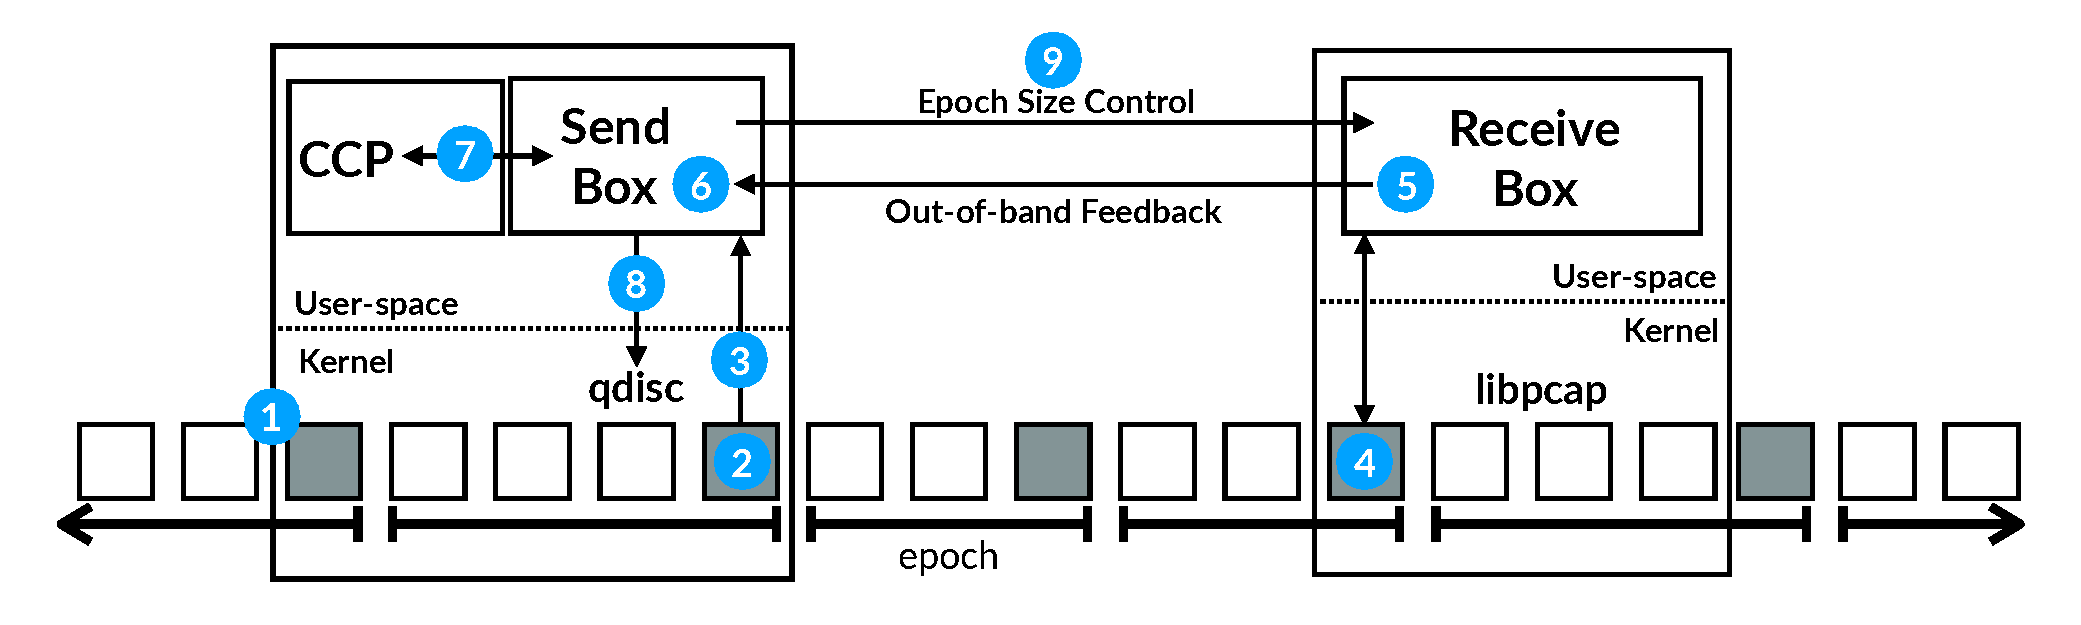
\includegraphics[width=2\columnwidth]{img/bundler-diagram}
    \caption{\name System Design}\label{fig:bundler}
\end{figure*}
To highlight the simplicity of our approach\footnote{and because we are lazy programmers}, we implement the inbox dataplane using Linux \texttt{tc}~\cite{tc}, and we limit our implementations of scheduling policy to those already widely available in the Linux kernel.
We patch the TBF queueing discipline (qdisc)~\cite{tbf} to enforce rates, and modify its ``inner\_qdisc'' to use a qdisc that enforces some scheduling policy.
Our patch to the TBF qdisc comprises $112$ lines of C.
The patch adds extra logging and the functionality to transmit feedback to the control plane using a netlink socket. 
Additionally, it removes one line in the rate update functionality to disable re-filling the token bucket on rate changes to prevent a penalty for frequent rate updates.

We implement the \inbox control plane to run in user-space in $1183$ lines of Rust. 
It uses \texttt{libnl} to communicate with the qdisc, and \texttt{libccp}~\cite{ccp} to communicate with the congestion control algorithm via Unix-domain sockets.
We use existing implementations of congestion control algorithms on CCP without modification\footnote{We discovered and patched a minor bug in the CCP Copa~\cite{copa} implementation.}; since CCP algorithms are already designed to receive network feedback asynchronously, they are a natural choice for our epoch-based measurement architecture.
It maintains the congestion control state of each bundle, but does not maintain (or observe) per-flow state.

We implement the \outbox using \texttt{libpcap} in $219$ lines of Rust. It listens for packets on the interface, checks for epoch packets, and sends the reports to the \inbox. 
The \outbox does not maintain any state.

Figure~\ref{fig:bundler} overviews the operation of our \name.

\begin{outline}
\1 blah
    \2 blah
        \3 When the qdisc observes an epoch-marked packet, it sends a message to the inbox process in userspace.
        \3 The userspace component of the inbox process manages the qdisc and acts as a CCP datapath. It communicates with the CCP congestion control algorithm via unix sockets or channels if the algorithm is run in a thread within the same process.
        \3 The userspace component of the inbox also listens for messages from the outbox. When it receives one, it updates the congestion control measurements and notifies CCP that new measurements are available.
        \3 The inbox enforces congestion windows by converting them to rates (by dividing by RTT). The inbox tells the qdisc to pace at rate min(set rate, cwnd effective rate).
    \2 We implement a scheduler with \an{something}
\end{outline}

\subsection{Fault Tolerance}\label{s:impl:ft}
\begin{outline}
\1 If outbox feedback is lost, the next outbox feedback that is successfully received at the inbox will determine the end of the measurement epoch.
    \2 The measurements will still be accurate, but they will end up being taken over a longer period than intended.
\1 The inbox dynamically sets the epoch duration to be (rate * rtt) rounded down to the nearest power of two. It then communicates the epoch duration to the outbox.
    \2 If this communication is lost, since the epoch duration is set to be a power of two, the inbox and outbox will still agree on a set of epoch packets.
\1 If the inbox crashes, the operator can remove it from the service chain, and performance will be no worse than it is today.
\1 If the outbox crashes, after a timeout period, the inbox will disable aggregation on the path and performance will be no worse than it is today.
\end{outline}

\subsection{Bundle Initialization}\label{s:impl:discovery}
\begin{outline}
\1 Discovery \an{should we even mention this? we don't implement it and it's not really important}
    \2 One practical concern in a \name deployment is how the inbox and outbox discover each others' presence.
    \2 The inbox should not apply pacing to packets which will not traverse an outbox: they may interfere with scheduling and consume unnecessary resources.
        \3 Instead, when the inbox encounters packets not included in a bundle group, it should immediately forward them without counting them against its statistics.
        \3 The inbox needs to know which packets are part of a bundle.
    \2 Also, the outbox needs to know what inbox to send feedback messages to.
    \2 Fortunately, with packet marking, this is straightforward. The inbox first assumes that all packets are not bundled, and transmits them normally.
    \2 The outbox first assumes all packets are bundled. Since it does not initially know of the existence of the inbox, it sends its feedback messages to the source IP address of the marked packet along with its IP address. As an optimization, the outbox could also include information such as the subnet of machines behind it.
        \3 When the inbox receives this feedback, it begins tracking congestion primitives for the bundle of flows destined for the outbox's subnet.
\end{outline}